\documentclass[11pt, a4paper]{article}

\usepackage{graphicx}
\usepackage[a4paper,top=3cm,bottom=2cm,left=2cm,right=2cm,marginparwidth=1.75cm]{geometry}
\usepackage[english]{babel}
\usepackage[utf8x]{inputenc}
\usepackage{subfig}
\usepackage{float}
\usepackage{amsmath}
\usepackage{amssymb}
\usepackage{mhchem}
\usepackage{hyperref}
\usepackage{tikz}
\usepackage{cancel}

\graphicspath{ {./images} }
\newcommand*{\qed}{\hfill\ensuremath{\quad\square}}%
\newcommand*{\rad}{\ensuremath{\,\text{rad}}}
\newcommand*{\R}{\ensuremath{\mathbb{R}}}
\newcommand*{\C}{\ensuremath{\mathbb{C}}}
\renewcommand*{\Re}{\operatorname{Re}}
\renewcommand*{\Im}{\operatorname{Im}}
\renewcommand*{\epsilon}{\varepsilon}
\renewcommand*{\phi}{\varphi}

\makeatletter
\renewcommand*\env@matrix[1][*\c@MaxMatrixCols c]{%
  \hskip -\arraycolsep
  \let\@ifnextchar\new@ifnextchar
  \array{#1}}
\makeatother

\newtheorem{theorem}{Theorem}

%------------------------------------------------
%Templates for images and figures
% \begin{figure}[h]
%   \centering
%   \subfloat[caption 1]{{
\includegraphics[width=30mm]{images/placeholder.png}}}%
%   \qquad
%   \subfloat[caption 2]{{
\includegraphics[width=30mm]{images/placeholder.png}}}%
%   \caption{Description}
% \end{figure}

% \begin{figure}[h]
%   \centerline{
\includegraphics[width=50mm]{images/placeholder.png}}
%   \caption{Description}
% \end{figure}

%Template for a simple table 
%\begin{table}[h]
%   \caption{Description} %title of the table
%   \centering % centering table
%   \begin{tabular}{l rr} % creating three columns
%     \hline\hline %inserting double-line
%     & & \\ [0.5ex] % Insert half line vertical spacing
%     \hline % inserts single-line
%     & & \\ 
%     & & \\
%     & & \\
%     & & \\
%   \hline % inserts single-line
%   \end{tabular}
%   \label{tab:hresult}
% \end{table}
%-----------------------------------------------

\begin{document}
\setcounter{equation}{0}
\setcounter{section}{6}

\section{WOP3B Lecture 7: Fatigue of screws (28/05/2020)}

\subsection{Fatigue strength as applied to screws}
Consider a bolt with a nut attached as show in the figure below.
\begin{figure}[h]
  \centerline{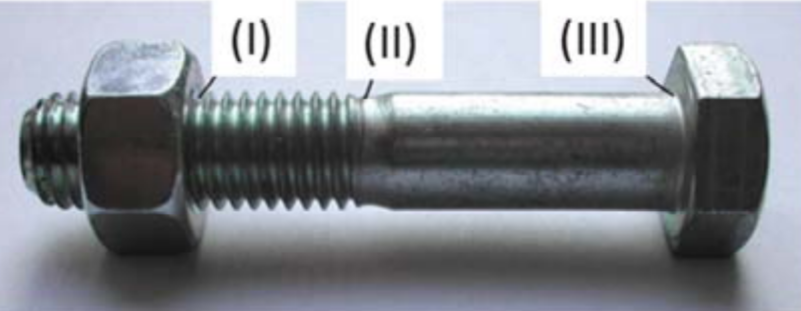
\includegraphics[width=80mm]{images/Bolt.png}}
  \caption{The bolt with 3 areas of interest denoted with $I$, $II$ and $III$}
\end{figure}
$I$ denotes the first thread engaged by the nut. $II$ denotes the thread run out at the bolt shank. $III$ denotes the fillet at the head of the bolt. The highest local stress in the bolt under a purely axial load will arise $I$ as $II$ and $III$ have been designed to be less critical then $I$ via an ISO norm. For static loading this would not matter. However, as we found previous lecture, stress concnetrations are much more important when considering dynamic loads.\\
\\
In practice we often see bolt failing at $III$ rather then at $I$. THis is because, in practice, loads are rarely purely in the axial direction. There is often times a bending load which increases the local stress at $III$ relative to the cross-section at $I$. Because of this bolts under dynamic loading are rarely threaded up untill the head of the bolt. This would increase the stress in $III$ making it the most critical point in the bolt.
\begin{figure}[h]
  \centerline{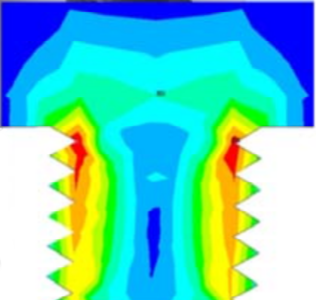
\includegraphics[width=50mm]{images/FEM.png}}
  \caption{FEM analysis of a bolt which is threaded up untill the head of the bolt}
\end{figure}


\subsection{Modified Goodman diagrams}
Bolts much like rotary equipment tend to reacht $10^7$ cycles fairly quickly.This is why we again turn to $SN$-diagrams, rather then $\epsilon N$-diagrams. However for bolts we are usually only interested in the endurance limit of the bolt relative to the mean stress. For this we introduce a new type of diagram, called a Modified Goodman Diagram (MGD) (sometimes also called Smith diagrams).
\begin{figure}[H]
  \centering
  \subfloat[General MGD]{{\includegraphics[width=60mm]{images/MGD_General.png}}}%
  \qquad
  \subfloat[applied to a bolt]{{\includegraphics[width=60mm]{images/MGD_bolts.png}}}%
  \caption{MGD in general in (a) and the MGD as applied to a bolt in (b)}
\end{figure}
The MGD gives the endurance limit on the vertical axis versus the mean load applied along the horizontal axis. From this type of diagram we can easily read that the endurance limit tends to go down when the mean applied load increases. Note that the applied load $R$ is given by:
\begin{equation}
  R = \frac{\sigma_{min}}{\sigma_{max}}
\end{equation}
Screws generally have a very low endurance limit. We can circumvent this by cleverly designing the screw joints.


\subsection{Case study: Screw joints}
Consider the 2 screw joints seen in the figure below:
\begin{figure}[H]
  \centerline{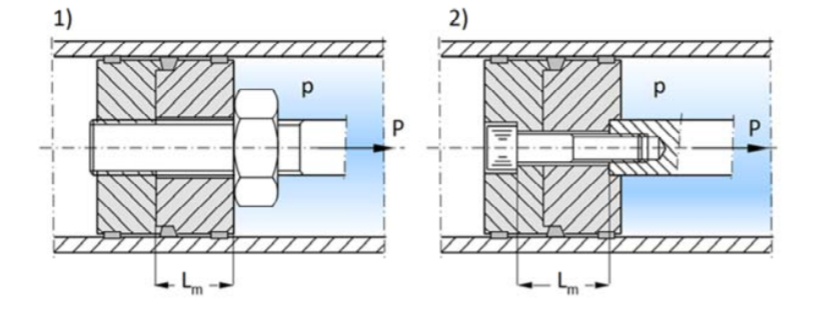
\includegraphics[width=120mm]{images/Bolt_2.png}}
  \caption{Two different designs that are being considered for the screw joint}
\end{figure}
Configuration 1 uses an M24-8.8 ($\sigma_e = 50\,MPa$) fastener. Configuration 2 uses an M12-8. ($\sigma_e = 45\,MPa$) fastener. For both designs $L_m=24\,mm$. We want to analyse which joint has the higher fatigue strength.\\
Consider the following FBD of a bolt:
\begin{figure}[h]
  \centerline{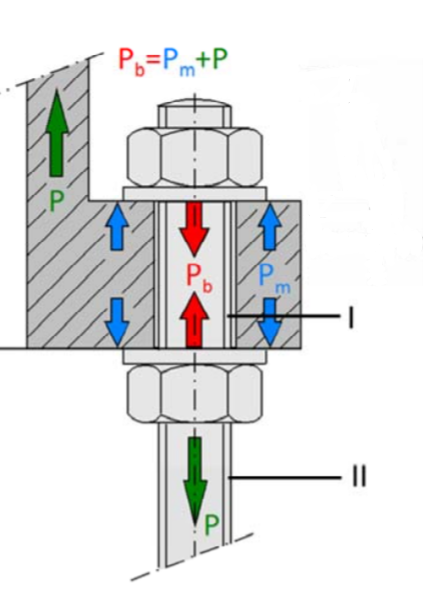
\includegraphics[width=50mm]{images/FBD.png}}
  \caption{The FBD a typical screw joint. $I$ is used to denote a pre-stressed area while $II$ is a non-prestressed area.}
\end{figure}
When the working load $P$ (green) is applied the strain increases. The force below the lowest nut increases, while the force exerted on the clamped material decreases. From this we can conclude that:
\begin{equation}
  P_b = P_m + P
\end{equation}
$P_m$ decreases while $P$ increases, thus the increase in the load on the screw ($P_b$) is \underline{smaller} then the increase in applied working load. We can use a joint stiffness diagram to find a maximum value for $P_b$. Looking at the FBD we find that for this situation $\frac{P_b}{P_m} = \frac{1}{3}$ and $\frac{P_b}{P} = \frac{1}{4}$. We define $P_b = C_m\cdot P$ where $C_m$ denotes the joint stiffness. From this we find that in this case $C_m = \frac{1}{4}$. Looking at the diagram leads to the conclusion that $P_b < F_{0.2}$ where $F_{0.2}$ is the force at $R_{p0.2}$.
\begin{figure}[h]
  \centerline{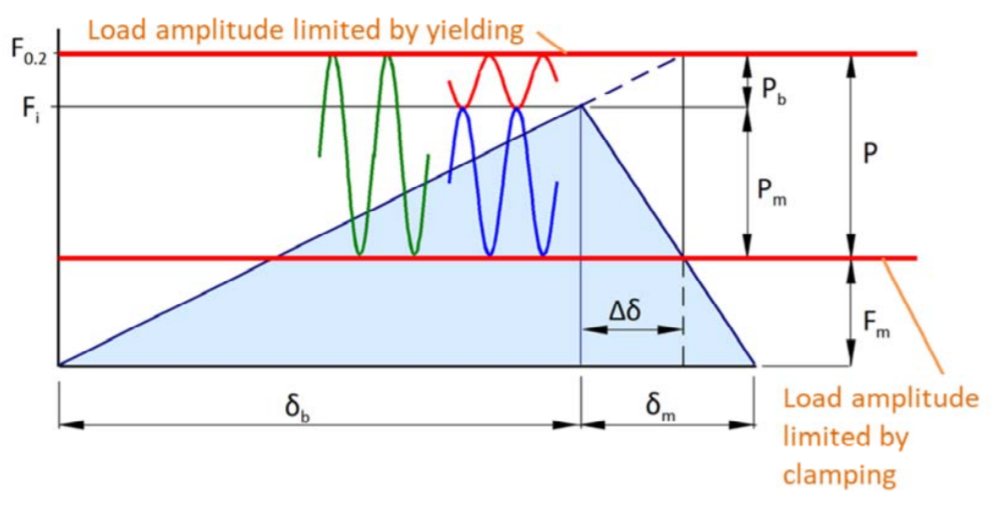
\includegraphics[width=80mm]{images/JSD.png}}
  \caption{Joint stiffness diagram of the screw}
\end{figure}
We can also use this diagram to find the maximum allowed value for $P_b$. There are $3$ fail mechanism which need to be considered.
\begin{enumerate}
  \item The bolt may not deform plastically, thus $P_b = F_{0.2} - F_i$ using $P_b = C_m\cdot P$ we find $P_{max,1}$.
  \item The clamping force is not allowed to be lower then $F_m$. Thus: $P_m = F_i - F_m$ with $P_b = \frac{\delta_m}{\delta_b}P_m$. We then find $P_{max,2}$ using $P_b = C_m\cdot P$.
  \item The endurance limit $P_b = 2\sigma_eA_s$ may not be exceeded. We use $P_b = C_m\cdot P$ to find $P_{max,3}$
\end{enumerate}
The actual maximum strength of a given joint is then given as:
\begin{equation}
  \text{min}(P_{max,1},P_{max,2},P_{max,3})
\end{equation}
Going back to our case study: We can see the second configuration can be loaded by approximatly twice as much.
\begin{figure}[H]
  \centerline{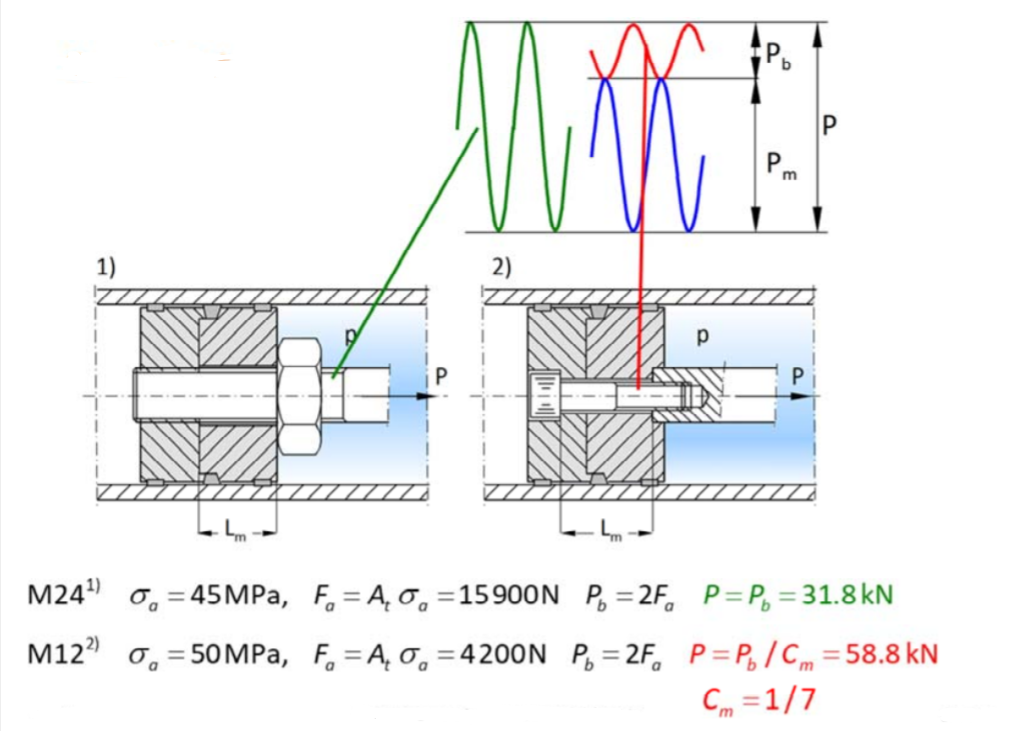
\includegraphics[width=120mm]{images/Bolts_3.png}}
  \caption{The information we found as applied to the 2 possible designs in the case study.}
\end{figure}


\subsection{The joint stiffness factor}
Quantifying the stiffnes of a regular bolt is fairly trivial using Hooke's law:
\begin{equation}
  \sigma = E\epsilon \Rightarrow k_L = \frac{AE}{L}
\end{equation}
This becomes a bit more complicated when it comes to computing the stiffness of a bolt clamping down. A pretty good rule of thumb is the following expression:
\begin{equation}
  C_m = \frac{P_b}{P} = \left( \frac{1}{1.5+0.289(L_m/d)} \right)^2  
\end{equation}
Where $C_m$ is the joint stiffness factor. We want $C_m$ to be small, thus a larger value for $L_m/d$ is beneficial. This means long thin bolts are preferred over shorter thicker ones when designing for fatigue life of a bolt.
\begin{figure}[H]
  \centerline{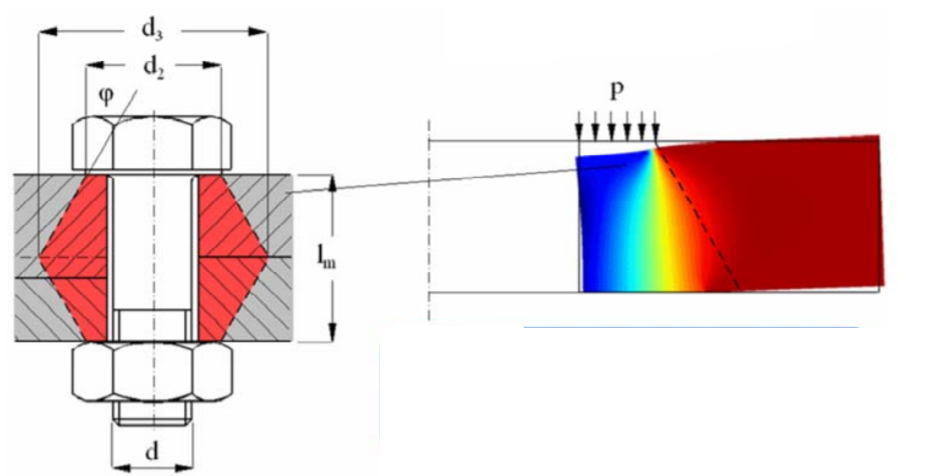
\includegraphics[width=120mm]{images/CM.png}}
  \caption{FEM analysis quantifying the stiffness factor $C_m$}
\end{figure}



\end{document}